% Hlavicka pro protokoly z fyzikalniho praktika.
% Verze pro: LaTeX
% Verze hlavicky: 22. 2. 2007
% Autor: Ustav fyziky kondenzovanych latek
% Ke stazeni: www.physics.muni.cz/ufkl/Vyuka/
% Licence: volne k pouziti, nejlepe k vcasnemu odevzdani protokolu z Vaseho mereni.

\documentclass[a4paper,11pt]{article}

% Kodovani (cestiny) v dokumentu: utf-8
%\usepackage[cp1250]{inputenc}	% Omezena stredoevropska kodova stranka, pouze MSW.
\usepackage[utf8]{inputenc}	% Doporucujeme pouzivat UTF-8 (unicode).

%%% Nemente:
\usepackage[margin=2cm]{geometry}
\newtoks\jmenopraktika \newtoks\jmeno \newtoks\datum
\newtoks\obor \newtoks\skupina \newtoks\rocnik \newtoks\semestr
\newtoks\cisloulohy \newtoks\jmenoulohy
\newtoks\tlak \newtoks\teplota \newtoks\vlhkost
\usepackage{amsmath}
\usepackage{mathtools}
\usepackage{graphicx}
\usepackage{multirow}
\graphicspath{ {./images/} }
%%% Nemente - konec.


%%%%%%%%%%% Doplnte pozadovane polozky:

\jmenopraktika={Fyzikální praktikum 2}  % nahradte jmenem vaseho predmetu
\jmeno={Artem Gorodilov}            % nahradte jmenem mericiho
\datum={19. ~října  2023}        % nahradte datem mereni ulohy
\obor={Astrofyzika}                     % nahradte zkratkou vami studovaneho oboru
\skupina={Čt 8:00}            % nahradte dobou vyuky vasi seminarni skupiny
\rocnik={II}                  % nahradte rocnikem, ve kterem studujete
\semestr={I}                 % nahradte semestrem, ve kterem studujete

\cisloulohy={5}               % nahradte cislem merene ulohy
\jmenoulohy={Magnetické pole} % nahradte jmenem merene ulohy

\tlak={976}                   % nahradte tlakem pri mereni (v hPa)
\teplota={21.8}               % nahradte teplotou pri mereni (ve stupnich Celsia)
\vlhkost={35}               % nahradte vlhkosti vzduchu pri mereni (v %)

%%%%%%%%%%% Konec pozadovanych polozek.


%%%%%%%%%%% Uzitecne balicky:
\usepackage[czech]{babel}
\usepackage{graphicx}
\usepackage{amsmath}
\usepackage{xspace}
\usepackage{url}
\usepackage{indentfirst}
\usepackage{listings}
\usepackage{subcaption}
\usepackage{caption}
\usepackage{tabularx}
\usepackage[labelformat=parens,labelsep=quad,skip=3pt]{caption}

%%%%%% Zamezeni parchantu:
\widowpenalty 10000 \clubpenalty 10000 \displaywidowpenalty 10000
%%%%%% Parametry pro moznost vsazeni vetsiho poctu obrazku na stranku
\setcounter{topnumber}{3}	  % max. pocet floatu nahore (specifikace t)
\setcounter{bottomnumber}{3}	  % max. pocet floatu dole (specifikace b)
\setcounter{totalnumber}{6}	  % max. pocet floatu na strance celkem
\renewcommand\topfraction{0.9}	  % max podil stranky pro floaty nahore
\renewcommand\bottomfraction{0.9} % max podil stranky pro floaty dole
\renewcommand\textfraction{0.1}	  % min podil stranky, ktery musi obsahovat text
\intextsep=8mm \textfloatsep=8mm  %\intextsep pro ulozeni [h] floatu a \textfloatsep pro [b] or [t]

% Tecky za cisly sekci:
\renewcommand{\thesection}{\arabic{section}.}
\renewcommand{\thesubsection}{\thesection\arabic{subsection}.}
% Jednopismenna mezera mezi cislem a nazvem kapitoly:
\makeatletter \def\@seccntformat#1{\csname the#1\endcsname\hspace{1ex}} \makeatother

\begin{document}

\thispagestyle{empty}

{
\begin{center}
\sf 
{\Large Ústav fyzikální elektroniky PřF MU} \\
\bigskip
{\huge \bfseries FYZIKÁLNÍ PRAKTIKUM} \\
\bigskip
{\Large \the\jmenopraktika}
\end{center}

\bigskip

\sf
\noindent
\setlength{\arrayrulewidth}{1pt}
\begin{tabular*}{\textwidth}{@{\extracolsep{\fill}} l l}
\large {\bfseries Zpracoval:}  \the\jmeno & \large  {\bfseries Naměřeno:} \the\datum\\[2mm]
\large  {\bfseries Obor:} \the\obor  \hspace{40mm}  {\bfseries Skupina:} \the\skupina %
%{\bfseries Ročník:} \the\rocnik \hspace{5mm} {\bfseries Semestr:} \the\semestr  
&\large {\bfseries Testováno:}\\
\\
\hline
\end{tabular*}
}

\bigskip

{
\sf
\noindent \begin{tabular}{p{3cm} p{0.6\textwidth}}
\Large  Úloha č. {\bfseries \the\cisloulohy:} \par
\smallskip
$T=\the\teplota$~$^\circ$C \par
$p=\the\tlak$~hPa \par
$\varphi=\the\vlhkost$~\%
&\Large \bfseries \the\jmenoulohy  \\[2mm]
\end{tabular}
}

\vskip1cm
\begin{minipage}[t]{1\textwidth}
\section{Zadání}
    Zaměřit horizontální složky intenzity magnetického pole Země Gaussovým magnetometrem.
    \par Změřit magnetickou odezvu feromagnetického materiálu (hysterezní smyčka).
\end{minipage}
    \par
    \vspace{10px}
    \begin{minipage}[t]{0.5\textwidth} 
    \section{Teorie}
        \subsection{Geomagnetické pole}
            Vlastnosti magnetického pole můžeme charakterizovat prostřednictvím intenzity magnetického pole, která je označována jako $H$. Tato vektorová veličina může být v každém bodě rozložena do dvou komponent. Jedna z těchto komponent směřuje horizontálně a druhá vertikálně. V našem měření se budeme zaměřovat na horizontální komponentu $H_z$.
            \par Horizontální složku magnetického pole Země lze měřit pomocí Gaussova magnetometru. Tento postup zahrnuje porovnání intenzity magnetického pole Země s intenzitou permanentního magnetu za použití magnetické střelky (kompasu), která ukazuje místní směr magnetického pole Země. Vzhledem k tomu, že pro reálný případ nemůžeme zanedbat rozměry permanentního magnetu, použijeme místo jednoho tyčového magnetu dva monopóly s magnetickým nábojem $+p$ a $-p$ umístěné ve vzdálenosti $l$ od sebe. Magnetická intenzita se poté dá vypočítat podle následujícího vztahu. Je však třeba zdůraznit, že magnetické monopóly jsou pouze myšlenkovými objekty a v reálném světě neexistují.
    \end{minipage}
    \hspace{10pt}
    \begin{minipage}[t]{0.5\textwidth} 
            K měření horizontální složky magnetického pole Země pomocí Gaussova magnetometru se využívají dvě Gaussovy polohy, které určují polohu permanentního magnetu vzhledem k střelce kompasu. Tyto Gaussovy polohy jsou znázorněny na obrázku (\ref{fig:gaussova poloha}).
            \vspace{10pt}
            \par 
            \centering
            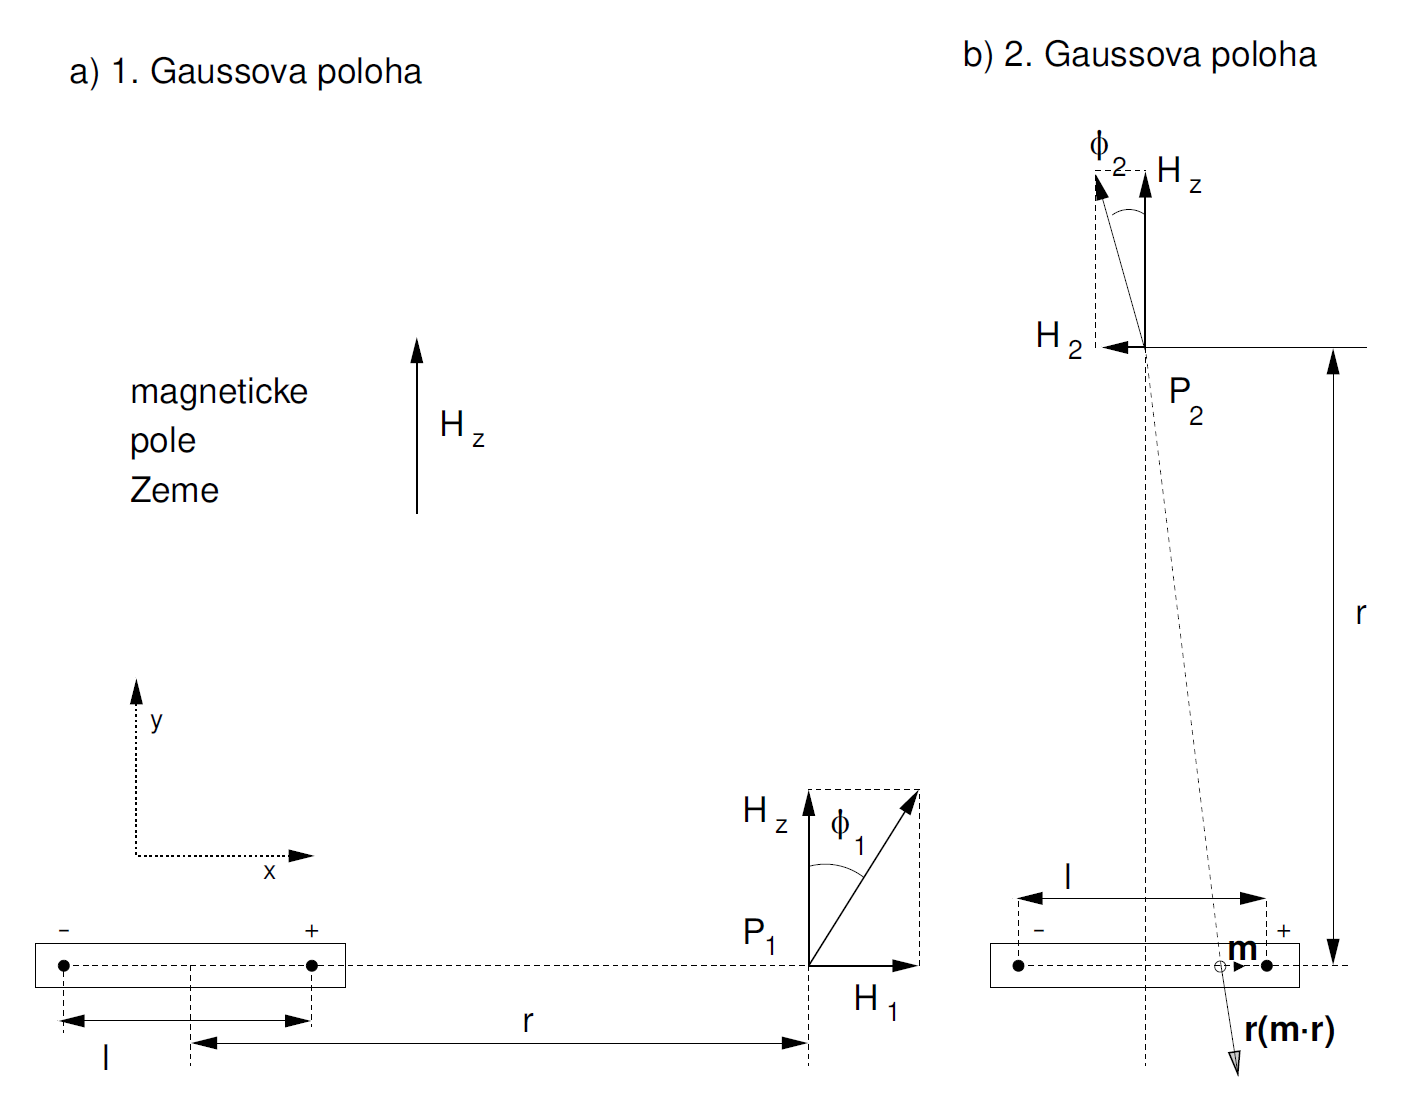
\includegraphics[scale=0.23]{gaussova poloha}
            \captionsetup{justification=centering, font=footnotesize}
            \captionof{figure}{Schéma experimentálního uspořádání. Magnetické pole v Gaussových polohách ($P_1$ první Gaussova poloha, $P_2$ druhá, a) resp. b)) v okolí permanentního tyčového magnetu a jeho skládání s magnetickým polem Země v místech magnetické střelky. Permanentní magnet je vždy orientován kolmo ke směru magnetického pole Země podél osy x. Úhlové výchylky magnetické střelky od jiho-severního směru v první a druhé poloze jsou označeny $\varphi_1$ resp. $\varphi_2$.}
            \label{fig:gaussova poloha}
            \vspace{10pt}
            \raggedright
    \end{minipage}
\newpage
    \begin{minipage}[t]{0.5\textwidth} 
            Poměr magnetického momentu magnetu k horizontální složce magnetického pole Země je roven: 
            \begin{equation}
                A = \frac{M}{H_z} = \frac{4 \pi r^3}{7} \left( \frac{3 tan\varphi_1}{2} +4 tan\varphi_2 \right)
            \end{equation}
            kde $r$ je vzdálenost mezi osou magnetické střelky a středem (těžištěm) tyčového magnetu, $\varphi_1$ je výchylka magnetky v první Gaussově poloze z jejího původního směru k magnetickému pólu Země, $\varphi_2$ je výchylka magnetky v druhé Gaussově poloze z jejího původního směru k magnetickému pólu Země a $\mu_0$ je permeabilita vakua.
            \vspace{10pt}
            \par Vyjádřením frekvence pomocí doby kmitů dostaneme rovnici:
            \begin{equation}
                B = MH_z = \frac{\pi^2 J}{\tau^2}
            \end{equation}
            kde $J$ je moment setrvačnosti magnetu a $\tau$ je doba kyvu magnetu.

            \begin{equation}
                \tau = \frac{T}{2}
            \end{equation}
            kde $T$ je perioda kmitů
            \begin{equation}
                J = \frac{m}{4} \left( R^2 + \frac{l^2}{3} \right)
            \end{equation}
            kde $m$ je hmotnost magnetu, $R$ je jeho poloměr a $l$ je jeho délka.
            \vspace{10pt}
            \par Horizontální složka zemského magnetického pole pak bude rovna: 
            \begin{equation}
                H_z = \sqrt{\frac{B}{A}}
            \end{equation}
            Magnetický moment magnetu se bude rovnat:
            \begin{equation}
                M = \sqrt{AB}
            \end{equation}
        \subsection{Magnetická odezva feromagnetického materiálu}
            Materiály můžeme klasifikovat do tří kategorií: diamagnetické, paramagnetické a feromagnetické. Feromagnetické materiály se výrazně liší od ostatních tím, že jsou schopny vykazovat magnetizaci i bez vnějšího magnetického pole. Tato magnetizace dosahuje své maximální hodnoty, když jsou všechny magnetické momenty v materiálu orientovány ve stejném směru, a tento stav nazýváme saturační (nasycená) magnetizace $M_s$. 
    \end{minipage}
    \hspace{10pt}
    \begin{minipage}[t]{0.5\textwidth} 
            I po odstranění vnějšího magnetického pole zůstává v materiálu remanentní (zbytková) magnetizace $M_r$. Dále můžeme určit velikost vnějšího pole, při kterém se celková magnetická indukce stane nulovou, a tuto hodnotu nazýváme koercitivní síla (nebo pole) $H_C$. Na základě této charakteristiky rozdělujeme materiály na magneticky měkké a magneticky tvrdé.
            \par Hysterezní smyčka je vidět na obrázku (\ref{fig:hyst}).
            \vspace{10pt}
            \par 
            \centering
            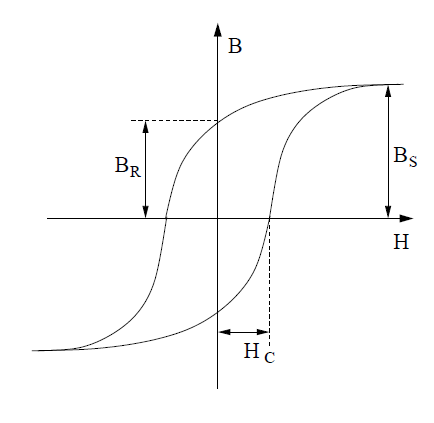
\includegraphics[scale=0.7]{hyst}
            \captionsetup{justification=centering, font=footnotesize}
            \captionof{figure}{Typický průběh magnetické hysterezní smyčky.}
            \label{fig:hyst}
            \vspace{10pt}
            \raggedright
            Testy provádíme na jádře s feromagnetickými vlastnostmi, které slouží jako společný prvek pro dvě cívky s odlišným počtem závitů (jde o transformátor). Transformátor je napájen střídavým elektrickým proudem a jeho zapojení odpovídá obrázku (\ref{fig:sheme}).
            \vspace{10pt}
            \par 
            \centering
            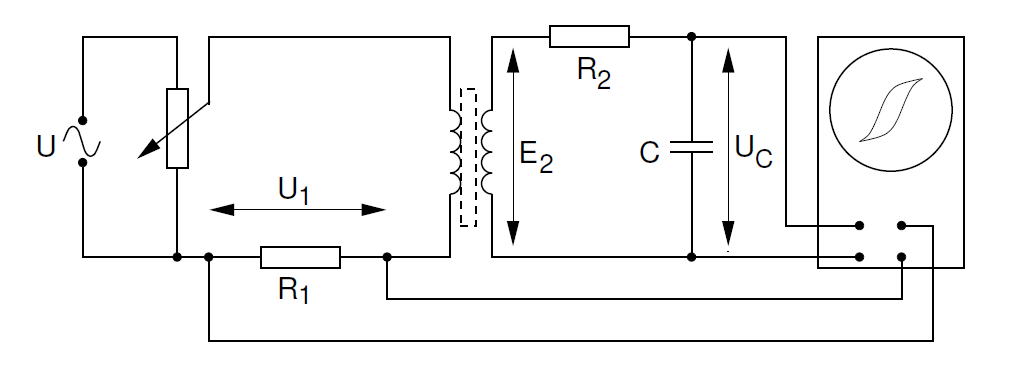
\includegraphics[scale=0.3]{sheme}
            \captionsetup{justification=centering, font=footnotesize}
            \captionof{figure}{Schéma obvodu pro měření magnetického pole ve feromagnetu.}
            \label{fig:sheme}
            \vspace{10pt}
            \raggedright
            Hodnota magnetické intenzity v toroidu se bude rovnat:
            \begin{equation}
                H(t) = \frac{N_1}{2 \pi r R_1} U_1(t)
            \end{equation}
            kde $N_1$ je počet závitů primárního vinutí, $r$ je poloměr jádra cívky, $R_1$ odpor rezistoru $R_1$ na obrázku (\ref{fig:sheme}) a $U_1$ je napětí na rezistoru $R_1$.
            \vspace{10pt}
    \end{minipage}
    \newpage
    \begin{minipage}[t]{0.5\textwidth} 
            \vspace{-50pt}
            Pokud je rozdíl vnitřního a vnějšího poloměru dostatečně malý:
            \begin{center}
                $r$ = $\frac{r_{min} + r_{max}}{2}$
            \end{center}
            kde $r_{min}$ vnitřní poloměr jádra a $r_{min}$ je vnější poloměr jádra.
            \vspace{10pt}
            \par Vztah pro magnetickou indukci:
            \begin{equation}
                B(t) = \frac{RC}{N_2 S_2} U_C(t)
            \end{equation}
            kde $R$ odpor rezistoru $R_2$, $C$ je kapacita kondenzátoru, $N_2$ je počet závitů sekundárního vinutí, $S_2$ je ploha průřezu jádra cívky a $U_C$ je napětí na cívce.
            \vspace{10pt}
            \par Plocha průřezu jádra cívky se rovná:
            \begin{equation}
                S_2 = h (r_{min} - r_{max})^2
            \end{equation}
            kde $h$ je ýška magnetu.
            \par Magnetizaci $M$ poté můžeme spočítat pomocí vztahu:
            \begin{equation}
                M = \frac{B}{\mu_0} - H
            \end{equation}
\section{Měření}  
        \subsection{Geomagnetické pole}
            Gaussův magnetometr inicializujeme v prvním Gaussově postavení, což znamená, že šipka směřující na sever je kolmá k pravítku, na němž je připevněn kompas. Poté umístíme tyčový magnet na kolejnici rovnoběžně s pravítkem a měříme změny úhlů v různých vzdálenostech od kompasu. Jakmile zaznamenáme odchylku kompasové střelky v jedné pozici, otočíme magnet o 180 stupňů a opět změříme změnu úhlu. Tento proces opakujeme pro tři různé pozice na jedné straně magnetometru a tři pozice na druhé straně. Tím získáme celkem 12 hodnot pro změny úhlů magnetické střelky.
            \par Následně magnet zavěsíme a vybočíme z rovnovážného stavu, abychom mohli měřit frekvenci harmonického pohybu.
            \par Změříme hodnoty úhlů pro dvě Gaussovy polohy a vypočítáme tečny těchto úhlů:
            \vspace{10pt}
            \par \centering
            \begin{tabular}{|c|c|c|c|}
                    \hline
                    $r$ [cm] & $\varphi_1_{zakl}$ [$^o$] & $\varphi_1_{otoč}$ [$^o$] & $tan\varphi_1$ \\
                    \hline
                    20 & 78 & 82 & 6(1) \\
                    \hline
                    30 & 57 & 61 & 1.6(1) \\
                    \hline
                    40 & 42 & 40 & 0.86(3) \\
                    \hline
                    -20 & 80 & 75 & 5(1) \\
                    \hline
                    -30 & 62 & 55 & 1.6(2) \\
                    \hline
                    -40 & 41 & 39 & 0.84(3) \\
                    \hline
                \end{tabular}
                \captionsetup{justification=centering, font=footnotesize}
                \captionof{table}{Naměřené úhly pro první Gaussovu polohu.}
                \vspace{20pt}
                \raggedright
    \end{minipage}
    \hspace{10pt}  
    \begin{minipage}[t]{0.5\textwidth} 
            \par \centering
            \begin{tabular}{|c|c|c|c|}
                    \hline
                    $r$ [cm] & $\varphi_2_{zakl}$ [$^o$] & $\varphi_2_{otoč}$ [$^o$] & $tan\varphi_2$ \\
                    \hline
                    20 & 74 & 77 & 3.9(4) \\
                    \hline
                    30 & 51 & 51 & 1 \\
                    \hline
                    40 & 33 & 34 & 0.66(1) \\
                    \hline
                    -20 & 73 & 79 & 4(1) \\
                    \hline
                    -30 & 53 & 54 & 1.35(3) \\
                    \hline
                    -40 & 35 & 33 & 0.68(3) \\
                    \hline
                \end{tabular}
                \captionsetup{justification=centering, font=footnotesize}
                \captionof{table}{Naměřené úhly pro druhou Gaussovu polohu.}
                \vspace{20pt}
                \raggedright
            Pak vypočítáme poměr magnetického momentu magnetu k horizontální složce magnetického pole Země $A$:
            \vspace{20pt}
            \par \centering
            \begin{tabular}{|c|c|}
                    \hline
                    $r$ [cm] & $A$ [m$^3$] \\
                    \hline
                    20 & 0.34(4)\\
                    \hline
                    30 & 0.36(1)\\
                    \hline
                    40 & 0.45(1)\\
                    \hline
                    -20 & 0.33(6)\\
                    \hline
                    -30 & 0.38(2)\\
                    \hline
                    -40 & 0.46(1)\\
                    \hline
                \end{tabular}
                \captionsetup{justification=centering, font=footnotesize}
                \captionof{table}{Poměr magnetického momentu magnetu k horizontální složce magnetického pole Země.}
                \vspace{20pt}
                \raggedright
            \par Měření průměru, délky a hmotnosti magnetu: 
            \begin{center}
                $d$ = 21.5(4) [mm]
                \par $l$ = 123.6(2) [mm]
                \par $m$ = 298.55(1) [g]
            \end{center}
            Z tabulek: 
            \begin{center}
                $\mu_0$ = $4\pi ~ 10^{-7}$ $\left[ \frac{N}{A^2} \right]$
            \end{center}
            \par Odtud zjistíme hodnotu $A$ podle vzorce (1): 
            \begin{center}
                $A$ = 0.39(6) [m$^3$]
            \end{center}
            Najděme moment setrvačnosti magnetu $J$ podle vzorce (4):
            \begin{center}
                $J$ = 3.89(1) $10^{-4}$ [$kg ~ m^2$]
            \end{center}
            Z měření: 
            \begin{center}
                $\tau$ = 6.4(2) [s]
            \end{center}
            Pak zjistíme hodnotu $B$ podle vzorce (2):
            \begin{center}
                $B$ = 9.3(6) $10^{-5}$ $\left[\frac{kg ~ m^2}{s^2} \right]$
            \end{center}
            Teď můžeme vypočítat horizontální složku magnetického pole Země $H_z$ podle vzorce (5) a magnetický moment magnetu $M$ podle vzorce (6):
            \begin{center}
                $H_z$ = 16(1) $\left[\frac{A}{m} \right]$
                \vspace{10pt}
                \par $M$ = 6.0(5) $10^{-6}$ $\left[A ~ m^2 \right]$
            \end{center}
    \end{minipage}
\newpage
    \begin{minipage}[t]{0.5\textwidth} 
        \subsection{Magnetická odezva feromagnetického materiálu}
            Z měření rozměrů jádra cívky vyplynuly následující hodnoty: 
            \begin{center}
                $r_{min}$ = 9.75(2) [mm]
                \vspace{5pt}
                \par $r_{max}$ = 14.50(2) [mm]
                \vspace{5pt}
                \par $h$ = 7.00(2) [mm]
            \end{center}
            Z tabulek: 
            \begin{center}
                $R_1$ = 83 [$\Omega$]
                \vspace{5pt}
                \par $R_2$ = 120 [k$\Omega$]
                \vspace{5pt}
                \par $C$ = 1.0 [$\mu F$]
            \end{center}
            \vspace{10pt}
            Křivku hystereze jsme získali z měření osciloskopem. Je vidět na obrázku (\ref{fig:hcurve}).
            \vspace{10pt}
            \par 
            \centering
            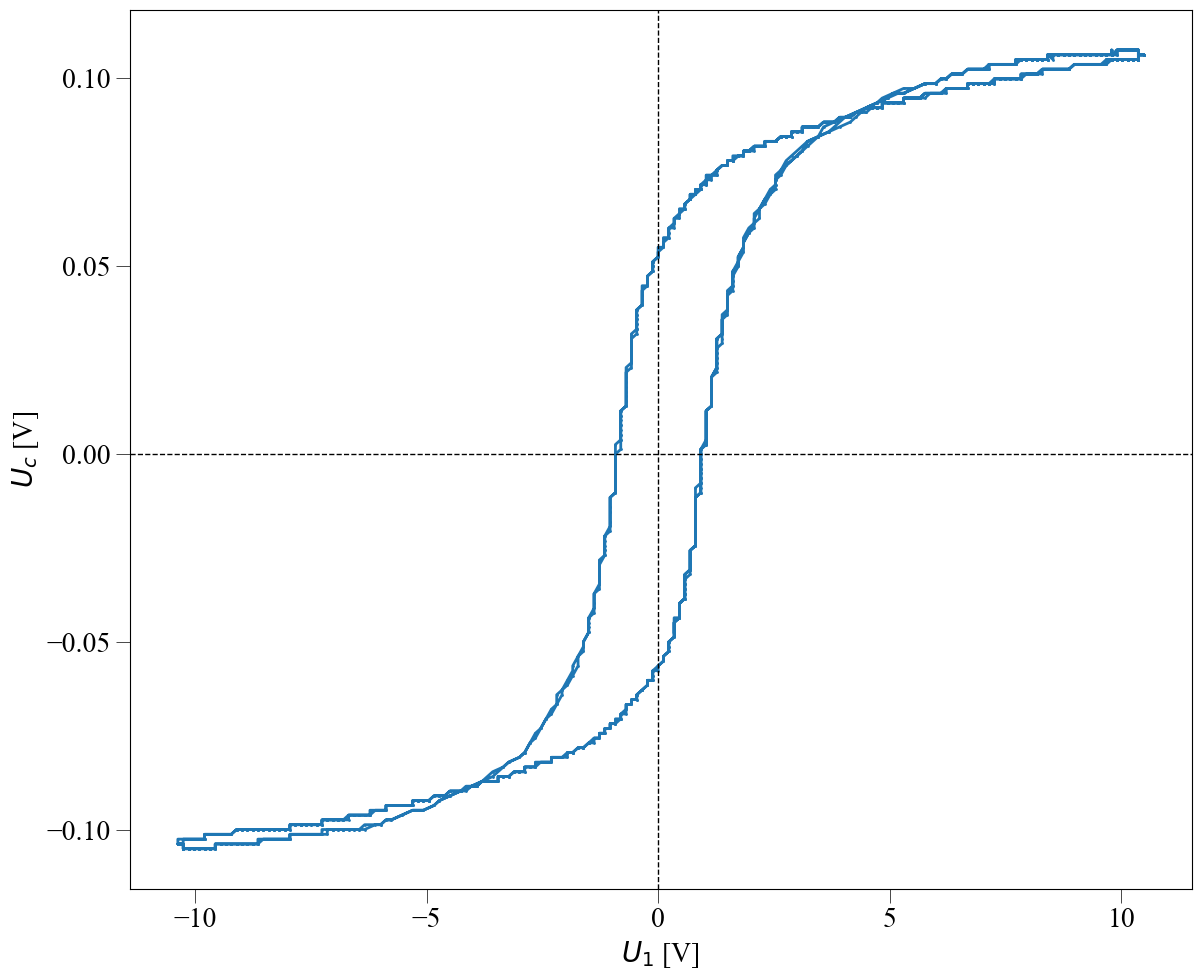
\includegraphics[scale=0.26]{hist_curve}
            \captionsetup{justification=centering, font=footnotesize}
            \captionof{figure}{Hysterezní křivka obvodu.}
            \label{fig:hcurve}
            \vspace{20pt}
            \raggedright
            Z grafu zjistíme hodnoty $U_1$, $U_C_r$ a $U_C_s$:
            \begin{center}
                $U_1$ = 0.92 [V]
                \vspace{5pt}
                \par $U_C_r$ = 0.053 [V]
                \vspace{5pt}
                \par $U_C_s$ = 0.11 [V], $U_1$ = 10.48 [V]
            \end{center}
            Plocha průřezu jádra cívky $S$ se zjistí ze vzorce (9):
            \begin{center}
                $S$ = 33.3(2) [mm$^2$]
            \end{center}
            Odtud zjistíme hodnotu magnetické intenzity $H_C$ v cívce podle vzorce (7): 
            \begin{center}
                $H_C$ = 37.83(4) $\left[ \frac{A}{m} \right]$
            \end{center}
    \end{minipage}
    \hspace{10pt}
    \begin{minipage}[t]{0.5\textwidth}
            Ze vzorce (8) zjistíme hodnoty magnetické injekce $B$ pro napětí $U_C_r$ a $U_C_s$:
            \begin{center}
                $B_r$ = 0.211(1) [T]
                \vspace{5pt}
                \par $B_s$ = 0.426(3) [T]
            \end{center}
            Dále zjistíme hodnoty remagnetizace a saturace podle vzorce (10): 
            \begin{center}
                $M_r$ =(1.68$\pm$0.01)$\times$ 10$^5$ [T]
                \vspace{5pt}
                \par $M_s$ = (3.39$\pm$0.02)$\times$ 10$^5$ [T]  
            \end{center}
            K výpočtu veličin a jejich nejistot byla použita knihovna Uncertinties pro Python: \href{pypi.org/project/uncertainties}. Kód je přiložen k protokolu. 
\section{Závěr}
        \subsection{Geomagnetické pole}
            Měření horizontální složky intenzity magnetického pole Země bylo provedeno pomocí Gaussova magnetometru. Vypočtená hodnota $H_Z$ = 16(1) $\left[\frac{A}{m} \right]$. Podle: NOAA Magnetic Field Calculator, by tato hodnota měla být přibližně $H_Z$ = 16.1 $\left[\frac{A}{m} \right]$.
            \par Dále byla získána hodnota magnetického momentu zkoumaného magnetu, která je $M$ = 6.0(5) $10^{-6}$ $\left[A ~ m^2 \right]$.
        \subsection{Magnetická odezva feromagnetického materiálu}
            Koercitivní pole, reziduální magnetizace a saturační magnetizace byly určeny analýzou hysterezní křivky, z níž byly odečteny hodnoty napětí $U_1$, $U_C_r$ a $U_C_s$. Tak byly získány následující výsledky: $H_C$ = 37.83(4) $\left[ \frac{A}{m} \right]$, $B_r$ = 0.211(1) [T] a $B_c$ = 0.426(3) [T].
            \par Saturace při napětí $U_1$ = 10.48 [V] se rovná $U_C_s$ = 0.11 [V]. Dále byla získána hodnota remagnetizace $M_r$ =(1.68$\pm$0.01)$\times$ 10$^5$ [T] a saturační magnetizace $M_s$ = (3.39$\pm$0.02)$\times$ 10$^5$ [T].
    \end{minipage}
\newpage
    \par K výpočtu chyb byl použit následující kód: 
    \begin{lstlisting}[language=Python, basicstyle=\tiny, breaklines=true, postbreak=\mbox{\textbackslashspace}]
        #Importing the libraries

        import matplotlib.pyplot as plt
        import numpy as np
        import pandas as pd
        from scipy import stats
        import uncertainties as u 
        from uncertainties import ufloat
        from uncertainties.umath import *
        from uncertainties import unumpy

        # Constants and values

        d = ufloat(21.5, 0.4)*10**(-3) #m
        l = ufloat(123.6, 0.2)*10**(-3) #m
        m = ufloat(298.55, 0.01)*10**(-3) #kg
        T = ufloat(6.409, 0.21697158032025) #s
        mu_0 = 4*np.pi*10**(-7) #N/A^2

        #Reading data

        data = pd.read_excel('data.xlsx')
        hist_u1 = pd.read_csv('TEK0000.csv')
        hist_uc = pd.read_csv('TEK0001.csv')

        #Geomagnetické pole

        tan_1 = []
        for ii,ID in enumerate(data['G1']):
            tan_1.append(ufloat(np.tan(np.radians((data['G1'][ii]+data['G1_rot'][ii])/2)), np.std(np.array([np.tan(np.radians(data['G1'][ii])),np.tan(np.radians(data['G1_rot'][ii]))]))))
        data['tan_1'] = tan_1
        
        tan_2 = []
        for ii,ID in enumerate(data['G2']):
            tan_2.append(ufloat(np.tan(np.radians((data['G2'][ii]+data['G2_rot'][ii])/2)), np.std(np.array([np.tan(np.radians(data['G2'][ii])),np.tan(np.radians(data['G2_rot'][ii]))]))))
        data['tan_2'] = tan_2
        
        data['A'] = ((4*np.pi*data['r']**3 / 7) * (3*data['tan_1']/2 + 4*data['tan_2'])) 
        
        A_values = []
        A_errors = []
        for ii,ID in enumerate(data['A']):
            A_values.append(data['A'][ii].nominal_value)
            A_errors.append(data['A'][ii].std_dev)
        
        A = ufloat(np.mean(np.abs(A_values)), np.sqrt(np.std(np.abs(A_values))**2 + np.mean(np.abs(A_errors))**2))
        print('A =', A, 'm^3')
        
        J = m/4 * ((d/2)**2 + (l**2/3))
        print('J =', J*10**4, 'e-4 kg m^2')
        
        B = (np.pi**2 * J) / (T**2)
        print('B =', B)
        
        H_z = sqrt(B/A) *10**(3)
        print('H_z =', H_z)
        
        M = sqrt(A*B) * 10**(-3)
        print('M =', M)
        
        print(data)

        #Magnetická odezva feromagnetického materiálu

        r_min = ufloat(9.75, 0.02)*10**(-3) #m
        r_max = ufloat(14.5, 0.02)*10**(-3) #m
        h = ufloat(7, 0.02)*10**(-3) #m
        
        R_1 = 83 #Ohm
        R_2 = 120*10**3 #Ohm
        N_1 = 260
        N_2 = 900
        C = 1 * 10**(-6) #F
        
        U_1 = 0.92 #V
        U_c_r = 0.0525 #V
        U_c_s = 0.1062 #V
        
        r = (r_min + r_max)/2
        
        H = N_1/(2*np.pi*r*R_1) * U_1
        print('H =', H)
        
        S = (r_max - r_min)*h
        print('S =', S)
        
        B_r = R_2*C/(N_2*S) * U_c_r
        print('B_r =', B_r)
        
        B_s = R_2*C/(N_2*S) * U_c_s
        print('B_s =', B_s)

        M_r = B_r/ mu_0 - H

        print('M_r =', M_r)

        M_s = B_s/ mu_0 - H

        print('M_s =', M_s)
    \end{lstlisting}  

\end{document}